\chapter{Regionally Containing Epidemics: Modelling Ash dieback}

Previously in Chapter \ref{ch5:dispersal-model}, we considered a generic $SIR$ model that spread via wind-borne dispersal. Constructing the dispersal model resolved the major problem witnessed in Chapter \ref{fig:ch4_uk_spread}, namely, the failure of the SLM to spread on a realistic host density. However, the findings of Chapter \ref{ch5:dispersal-model} lacked biological specificity and thus, came short of adding tangible value to the betterment of plant health. As such, this chapter will adopt a simplified model of ash dieback–based on the dispersal model–and utilised to develop an epidemic control strategy.

There has been a great deal of work carried out into the nature of control in plant and tree-based epidemics\footnote{See section \ref{chapter2:plant-ecologoy} for a review on the control in plant-based epidemics.}. In particular, the spatial structure of plant-hosts is an essential factor when considering how to manage an outbreak \cite{spatial-control-optimisation, control-heterogeneous-landscapes}. The accepted paradigm of control typically considers infected tree removals over a relatively small spatial scale, near infected hosts \cite{WEBIDEMICS}, or more broadly, ahead of the wavefront \cite{large-scale-control}. However, landscape-level epidemic control, based solely on the structure of large-scale spatial distribution of hosts incorporating topography, has yet to be explored in-depth.\\

As such, in this chapter, we will examine how host-heterogeneity, under the influence of a pathogen, can give rise to natural pinch-points and fault lines in the spatial distribution of hosts. Population pinch points may give rise to a bottleneck in the epidemic spread, which in principle, may be exploited with targeted tree felling to fragment the host population with minimised effort. In essence, a strategy of 'regional containment', targeting the local wind-based pathogen dispersal mechanism, is formulated and scaled up over large spatial scales. Similar concepts for crop and livestock diseases have been outlined \cite{PAPAIX201435, GILIOLI20131, Gilligan-disease-management}, however, to our knowledge, this has not been generalised to tree population distributions over large spatial scales.\\


A simplified $SEIR$-type model of ash dieback is developed to demonstrate this control strategy, alongside an appropriate definition of the reproductive ratio\textemdash denoted by $R_0$.  The value of $R_0$ is projected onto the map of ash tree canopy cover in GB, as given by \cite{hill.data}. From the $R_0$ maps we construct, a simple notion of epidemiological connectivity can be defined and visualised through a susceptible '$R_0$-cluster' over the population of GB ash trees. This leads us to develop a heuristically-based fragmentation algorithm. As we define it, fragmentation considers which locations in the population, if artificially taken below $R_0 = 1$ through felling, would disrupt epidemiological connectivity\textemdash, thus leading to containment. Epidemic containment in the largest $R_0$-cluster is then analysed and shown to be most applicable over a specific range of infectivity parameters.

\section{Methods}

\subsection{A simplified model of ash dieback}
% R0 is the measure used to capture the pathogens ability to invade
% Q: what is the relationship between the mortality ratio (or final fraction of infected hosts) ? 
% Ash dieback is known to sporulate in the summer months... therefore...
% we contend the SnIEmR model, considered over one sporulation peak, is a simplistic implementation of the SEIR-based model needed to compute an invasion threshold that represent the infection dynamics ash dieback. 
% By SnEmIR model has beneft of being readily extended or adapted to incorporate more biological realism, by virtue of splitting the E and I into multiple compartments.
% If R0 was considered over a larger time-scale, host-regrowth would need to be integrated into the model
% Furthermore, measuring R0 over a larger time-scale could over, or underestimate, the degree to which a response would need to be undertaken in the response time-window. 
% Typically an infected ash tree may expect to survive for around x years before death, this time-scale is beyond what we consider here - why ?
% sporulation has been fitted to an .... distribution \citations...
% Fitting data to the early phases of an epidemic has been shown to give large differences in the final-size epidemic, or severity \cite{doi:10.1094/PHYTO-12-10-0338}. However, we .... xyz cover all basis of using a one-season approximation. <- this leads to a risk-based argument in which we could capture a 2nd-order R0 which does, xyz. We mainly interested in a pathogens ability to invade.


\blindtext

\subsection{Defining $R_0$}

\begin{itemize}
    \item see for a review on how R0 is calculated \cite{perspectives-on-r0}, we use method x in order to estimate and inform R0
    \item $R_0$ is a complex function which changes in time, to this end, the next generation operator is used to derive a value for $R_0$ \cite{doi:10.1098/rsif.2009.0386}. In order to inform the value of $R_0$ we do xy and z...
    \item Although it is hard to enforce a true $R_0$ value, the most important feature introduced from the definition is a threshold from which we can see if a local invasion is likely to take place.
    \item Since the number of susceptible hosts is fixed, without replacement, the number of susceptible hosts will continually decrease in time in the case of an epidemic. Given the strong spatial component in the model we expect that measuring $R_0$ as-per this definition will give an under-estimate for later times when few susceptible trees remain. Likewise, for earlier times when susceptible neighbours are plentiful $R_0$ will yield an upper estimate for the pathogen. In order to characterise the pathogen in this model, we take the upper bound defined between the $1^{st}-2^{nd}$ generations. This simplification represents a worst-case scenario and the mean value of $R_0$ would be lower for later times when there are less trees available to infect. But most importantly, the threshold of transmission $R_0>1$ is reliable captured \textit{during the initial stage of infection}.
    \item $R_0$ can be fully characterised by a growth rate \cite{R0-construct}. That is, the growth factor per generation.
    
\end{itemize}

\textcolor{red}{Improvements to Chapter \ref{chapter:regional-containment1}}
\begin{enumerate}
    \item
\end{enumerate}

In this Chapter aspects of the sub-grid model are improved.//
\section{The biology of Ash dieback} % why not remain with Oak?
\begin{itemize}
    \item review: \cite{ash-dieback-costs}
    \item review: \cite{doi:10.1111/1365-2745.13383}
    \item review: \cite{ash-tree1}
\end{itemize}

\subsection{Constructing $R_0$-maps}
\begin{figure}
    \centering
    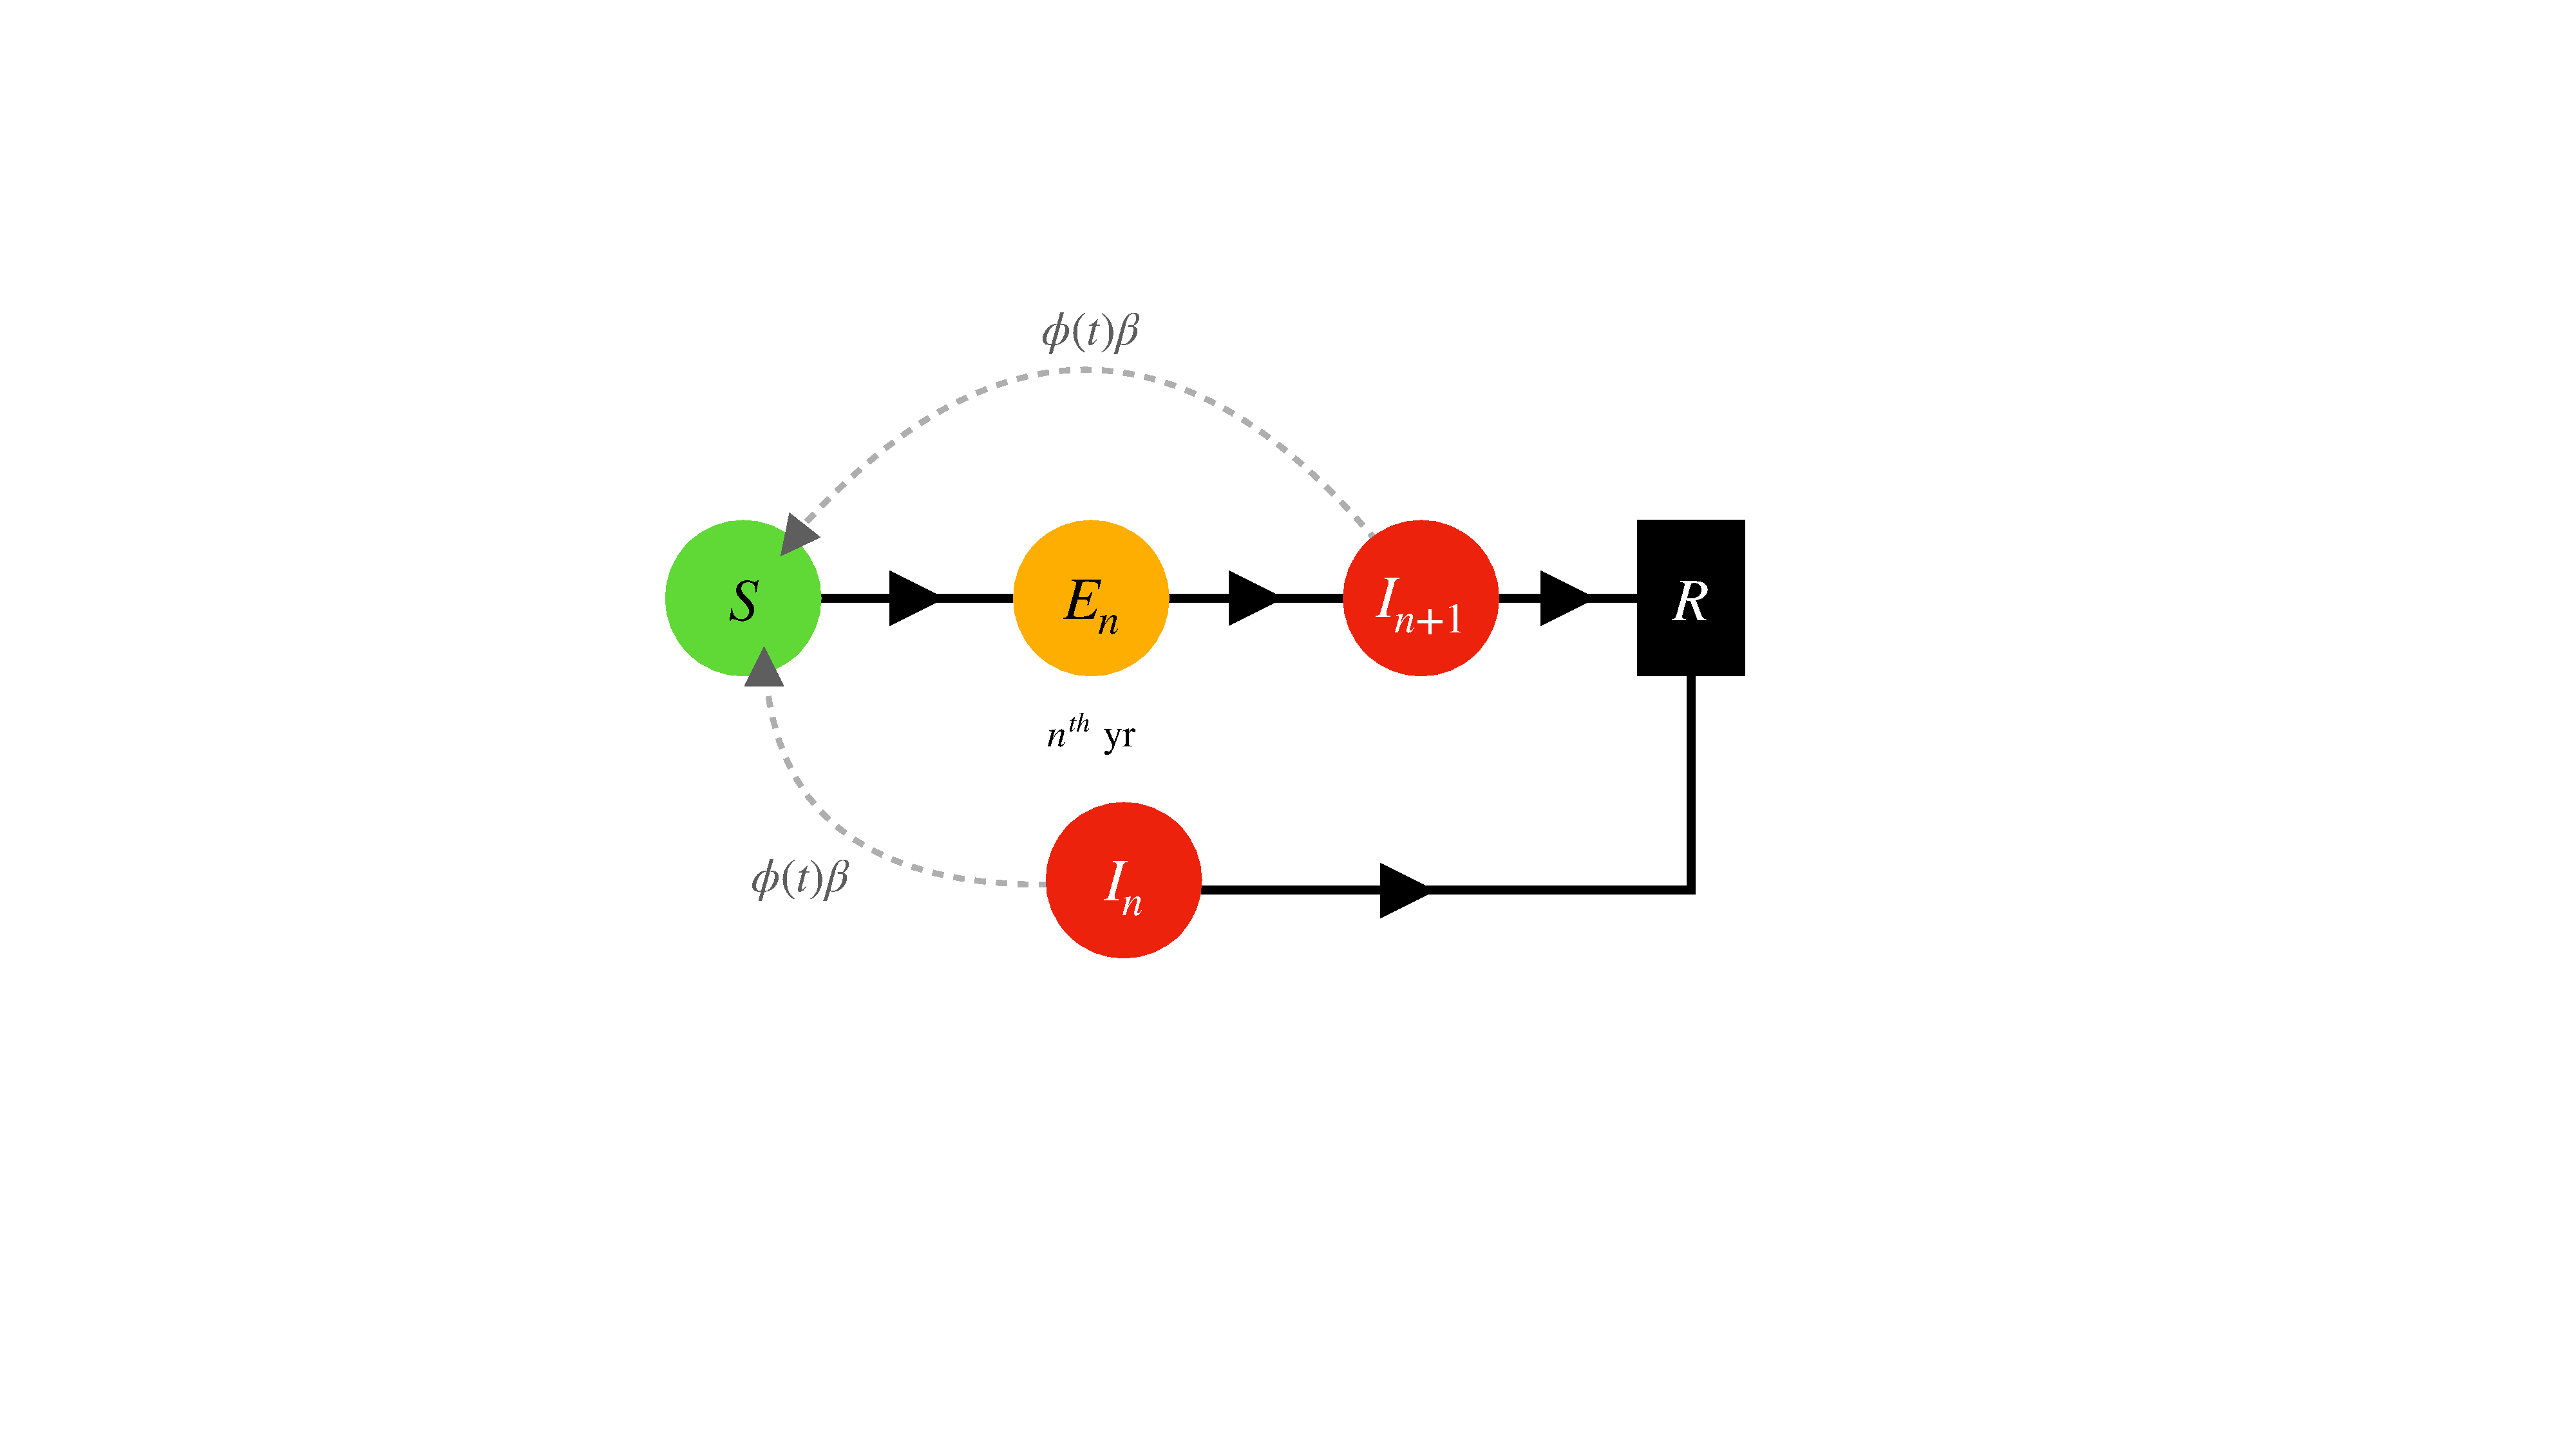
\includegraphics[scale=0.30]{chapter6/figures/fig1.pdf}
    \caption{Contact-traced $R_0$, the 'true' $R_0$. Tracking the history of all infected trees allows us to count how many infections are produced for each infectious tree over a simulation. At $t=0$, a handful of ($0^{th}$-generation) infections are positioned randomly throughout the domain. The quantity $R_0$ is defined as the mean number of secondary infections produced over all generations.}
    \label{fig:my_label}
\end{figure}

\begin{figure}
    \centering
    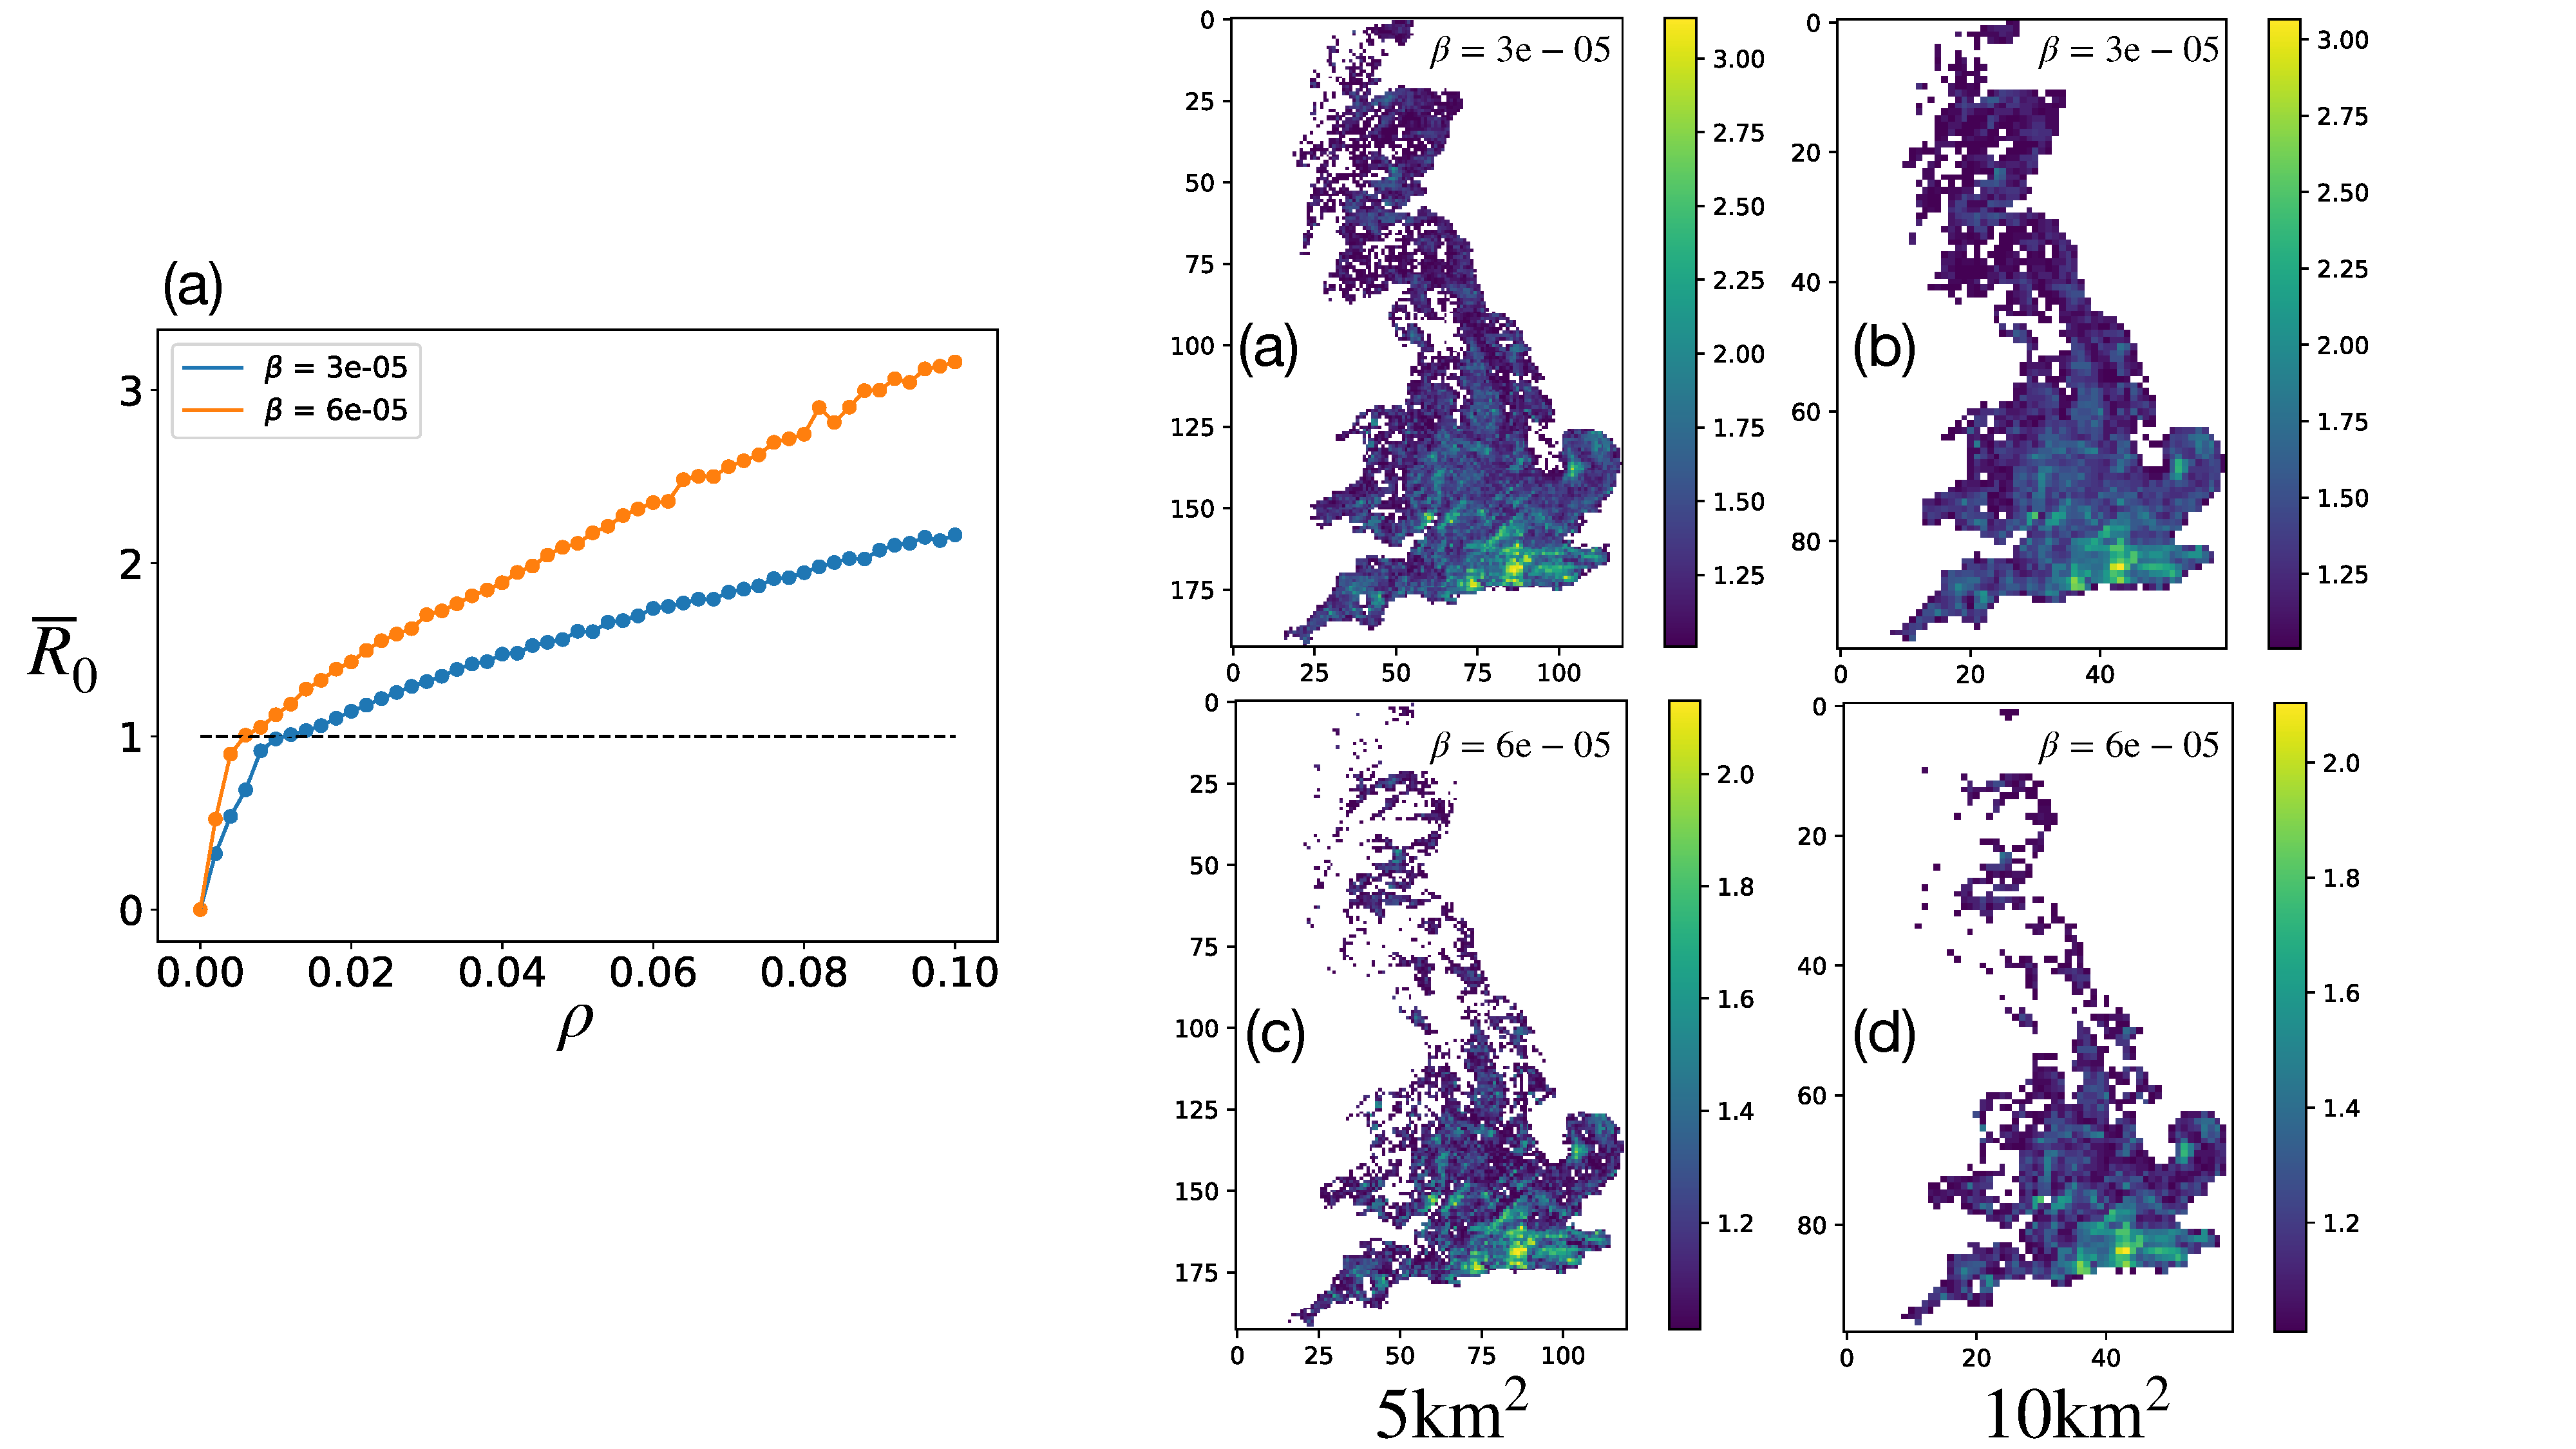
\includegraphics[scale=0.25]{chapter6/figures/fig2.pdf}
      \caption{(a) Ensemble-averaged $R_0$ between two values of $\beta$, for Gaussian dispersal of $\ell=1.6\mathrm{km}$. (a-b) $R_0$-map for $\beta=3\mathrm{e}-05$, coarse-grained at $5$, $ 10\mathrm{km^2}$. (c-d) $R_0$-map for $\beta=6\mathrm{e}-05$.}
    \label{fig:my_label}
\end{figure}

\section{Chapter summary}

\textbf{Model improvements...}
\begin{itemize}
    \item \textcolor{red}{At the small scale we have a uniform population. However for larger scales we have considerable spatial heterogeneity.}
    \item some regions can sustain an epidemic and some cannot, we assume that $R_0>1$ is the threshold separating these regimes.
    \item Looking at \cite{R0-perc-ref}, it makes me think our notion of $R_0$ is pretty simplistic. We only measure the local-level $R_0$. We do not consider $R_0$ from patch to patch. What scale we measure $R_0$ has a huge impact on what the result is. Could we rank land-patches not only on there local $R_0$ level, but also on the impact they have on there immediate neighbours ? This would, in theory be an improvement to the clustering algorithm.
    \item The algorithm to target not only the critically connecting patches, but also find fragmenting lines which minimise risk at the landscape-level ? Incorporating the local impact a particular patch may have on its neighbours.
    \item introduce the regime of pathogen spread we are interested in, we are not modelling continental long-range spread via upper atmosphere, nor are we interested in long-range human trade networks. We are interested in dispersal at the local level whereby passive means of wind, soil and or insects/animals. 
\end{itemize}

There are many pathways a pathogen can use to spread through a landscape, including long-range dispersal, mediated through either human-trade networks %
\cite{hulme2009trade, banks2015role, chapman2017global} or dispersal in the upper atmosphere \cite{westbrook1999atmospheric, isard2005principles}.

Here, we targeted interested in local-level dispersal via the landscape-level population structure. Dispersal over this small spatial-scale is thought to predominately occur passively through wind, however other  means of dispersal exist such as soil and or insects.

To our knowledge, $R_0$ has not been estimated for Ash dieback, or indeed for any large deciduous tree species, unlike for some crop-based pathogens \cite{segarra2001epidemic}. The lack of $R_0$-estimates made it hard to scrutinize which $\beta$-valued $R_0$-map would be likely to reflect reality. This gap in the body of literature is hardly surprising given the complexity of measuring time-varying infectivity rates \cite{13-challenges}. Thus, as it stands, our results hint-towards the utility of landscape-level control but come short of definitive proof.

aspects of our findings. 


